\documentclass[letter]{article}

\usepackage{MD_estilo}

\nombre{Matías Duhalde} % Aqui va el nombre del alumno
\lista{-} % Aqui va el numero de lista
\numtarea{1} % Aqui va el número de la tarea

\sigla{IIC2223} % Aqui va la sigla del curso
\curso{Teoría de Autómatas y Lenguajes Formales} % Aqui va el nombre del curso
\semestre{2} % Aqui va el semestre del curso
\ano{2021} % Aqui va el año del curso


\begin{document}
	
\begin{pregunta}{1} % Aqui se coloca el número de la pregunta

Sabemos que si $L$ es un lenguaje regular, existe un DFA que acepta el dicho lenguaje. En otras palabras, existe un DFA $A = (Q, \Sigma, \delta, q_0, F)$ tal que $L(A) = L$.

Se define la DNF $A' = (Q, \Sigma, \delta, q_0, F')$, donde $F'$ se define como
\begin{align*}
    F' =  \{ q \in Q \ | \ \delta(q, x) = p, p \in F,  x \in \Sigma \}
\end{align*}
En otras palabras, $F'$ es el conjunto de estados tales que tienen una transición a un estado final en la máquina $A$ que acepta $L$. Se quiere demostrar que $L - 1 = L(A')$, es decir, $A'$ define el lenguaje $L - 1$. \\

$\mathbf{L - 1 \subseteq L(A')}$ \\

Sea $w = a_1 a_2 ... a_n$, tal que $w \in \Sigma^*$ y $w \in L - 1$. Por definición de $L - 1$, existe un $a \in \Sigma$ tal que $w \cdot a \in L$. A continuación, se muestra una ejecución de $w \cdot a$ sobre el DFA $A$ que posee el lenguaje $L$:
\begin{align*}
    q_0 \rightarrow p_1 \rightarrow ... \rightarrow p_{n-1} \rightarrow p_n
\end{align*}
Donde $p_i \in Q$ para todo $i \leq n$, y $p_n \in F$.

$A$ tiene la misma función de transición $\delta$, estado inicial $q_0$, alfabeto $\Sigma$, y estados $Q$ que $A'$, por lo que para un mismo input, sus ejecuciones son equivalentes, y la ejecución de $A$ y $A'$ para el input $w \cdot a$ son idénticas. Si ejecutamos $A'$ con $w$, el estado final de la ejecución será $p_{n-1}$. Por definición de $A'$, $p_{n-1} \in F'$, por lo que la ejecución también será de aceptación, y $w \in L(A')$. \\


$\mathbf{L(A') \subseteq L - 1}$ \\

Por contradicción, supongamos que existe un $w = a_1a_2...a_n$, tal que $w \in L(A')$, pero $w \notin L - 1$. Entonces, $w$ posee la siguiente ejecución de aceptación en $L(A')$:
\begin{align*}
    q_0 \rightarrow p_1 \rightarrow ... \rightarrow p_{n-1} \rightarrow p_n
\end{align*}
Ahora, por definición de $L - 1$, si $w \notin L - 1$, entonces $w \cdot a \notin L$, para cualquier $a \in \Sigma$. La máquina $A$ que posee el lenguaje $L$ tendría la siguiente ejecución sobre $w \cdot a$.
\begin{align*}
    q_0 \rightarrow p_1 \rightarrow ... \rightarrow p_n \rightarrow p_{n + 1}
\end{align*}
Esta ejecución rechaza $w \cdot a$, por lo que $p_{n + 1} \notin F$. Aquí, se pueden dar dos casos: 
\begin{enumerate}
    \item Existe otro $x \in \Sigma$ para el cual $A$ acepta $w \cdot x$. Aquí se evidencia una contradicción, debido a que si existe otro $x$, entonces, por definición de $L - 1$, $w \in L - 1$.
    \item No existe ningún otro $x \in \Sigma$ para el cual $A$ acepta $w \cdot x$. En este caso, surge otra contradicción, debido a que los estados finales de $A'$ fueron definidos de la siguiente manera: $F' =  \{ q \in Q \ | \ \delta(q, x) = p, p \in F,  x \in \Sigma \}$, por lo que sería imposible que $p_{n} \in F'$ y $w \in L(A')$.
\end{enumerate}

Por lo tanto, $w$ \textbf{debe} pertenecer al lenguaje $L - 1$, y en consecuencia, $L(A') \subseteq L - 1$. Dado que se encontró un DFA $A'$ que posee el lenguaje $L - 1$ (para $L$ regular), se puede concluir que $L - 1$ es un lenguaje regular. \qed

\end{pregunta}

\begin{pregunta}{2}

\subsection*{Parte 1}

\begin{align*}
    L_1 = \{ \vec{v_1} \vec{v_2} ... \vec{v_n} \in (\{0, 1\}^3)^* \ \vert \ n \geq 1 \land \Sigma^n_{i=1} \vec{v_i} = [ \ 0 \ 0 \ 0 \ ]^t \}
\end{align*}

Para definir un autómata capaz de aceptar este lenguaje, primero se definen 3 autómatas

\begin{center}
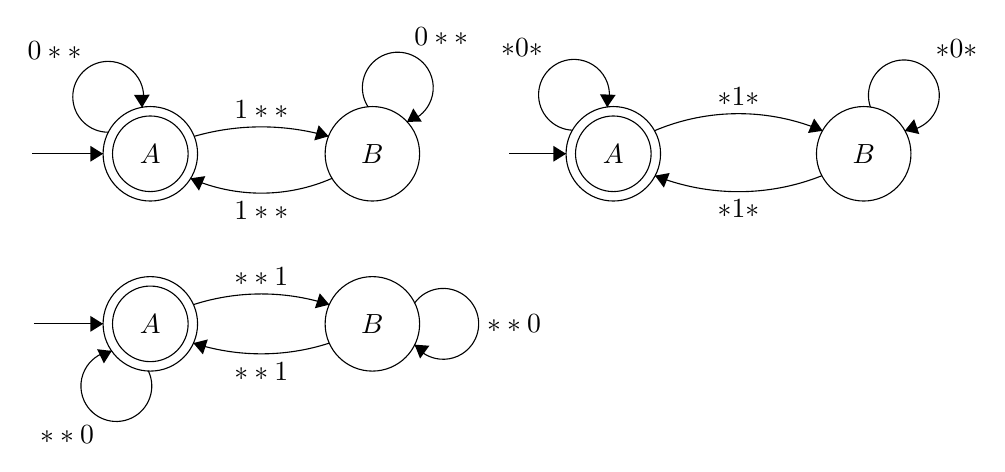
\begin{tikzpicture}[scale=0.2]
\tikzstyle{every node}+=[inner sep=0pt]
\draw [black] (15.9,-23.3) circle (3);
\draw (15.9,-23.3) node {$A$};
\draw [black] (15.9,-23.3) circle (2.4);
\draw [black] (30,-23.3) circle (3);
\draw (30,-23.3) node {$B$};
\draw [black] (15.9,-34.1) circle (3);
\draw (15.9,-34.1) node {$A$};
\draw [black] (15.9,-34.1) circle (2.4);
\draw [black] (30,-34.1) circle (3);
\draw (30,-34.1) node {$B$};
\draw [black] (45.3,-23.3) circle (3);
\draw (45.3,-23.3) node {$A$};
\draw [black] (45.3,-23.3) circle (2.4);
\draw [black] (61.2,-23.3) circle (3);
\draw (61.2,-23.3) node {$B$};
\draw [black] (8.4,-23.3) -- (12.9,-23.3);
\fill [black] (12.9,-23.3) -- (12.1,-22.8) -- (12.1,-23.8);
\draw [black] (18.683,-22.194) arc (106.09342:73.90658:15.391);
\fill [black] (27.22,-22.19) -- (26.59,-21.49) -- (26.31,-22.45);
\draw (22.95,-21.09) node [above] {$1**$};
\draw [black] (27.446,-24.857) arc (-66.30934:-113.69066:11.19);
\fill [black] (18.45,-24.86) -- (18.99,-25.64) -- (19.39,-24.72);
\draw (22.95,-26.3) node [below] {$1**$};
\draw [black] (8.5,-34.1) -- (12.9,-34.1);
\fill [black] (12.9,-34.1) -- (12.1,-33.6) -- (12.1,-34.6);
\draw [black] (38.7,-23.3) -- (42.3,-23.3);
\fill [black] (42.3,-23.3) -- (41.5,-22.8) -- (41.5,-23.8);
\draw [black] (47.912,-21.837) arc (112.97745:67.02255:13.674);
\fill [black] (58.59,-21.84) -- (58.05,-21.06) -- (57.66,-21.98);
\draw (53.25,-20.25) node [above] {$*1*$};
\draw [black] (58.549,-24.692) arc (-68.30313:-111.69687:14.332);
\fill [black] (47.95,-24.69) -- (48.51,-25.45) -- (48.88,-24.52);
\draw (53.25,-26.21) node [below] {$*1*$};
\draw [black] (18.635,-32.88) arc (107.91521:72.08479:14.029);
\fill [black] (27.27,-32.88) -- (26.66,-32.16) -- (26.35,-33.11);
\draw (22.95,-31.7) node [above] {$**1$};
\draw [black] (27.267,-35.322) arc (-72.04373:-107.95627:14.002);
\fill [black] (18.63,-35.32) -- (19.24,-36.04) -- (19.55,-35.09);
\draw (22.95,-36.5) node [below] {$**1$};
\draw [black] (29.728,-20.324) arc (212.96249:-75.03751:2.25);
\draw (34.37,-16.46) node [above] {$0**$};
\fill [black] (32.2,-21.27) -- (33.14,-21.26) -- (32.6,-20.42);
\draw [black] (61.63,-20.343) arc (199.46741:-88.53259:2.25);
\draw (67.09,-17.24) node [above] {$*0*$};
\fill [black] (63.81,-21.84) -- (64.73,-22.05) -- (64.4,-21.1);
\draw [black] (32.68,-32.777) arc (144:-144:2.25);
\draw (37.25,-34.1) node [right] {$**0$};
\fill [black] (32.68,-35.42) -- (33.03,-36.3) -- (33.62,-35.49);
\draw [black] (15.775,-37.086) arc (25.34226:-262.65774:2.25);
\draw (10.61,-40.53) node [below] {$**0$};
\fill [black] (13.45,-35.82) -- (12.52,-35.71) -- (12.95,-36.61);
\draw [black] (13.244,-21.931) arc (270.46923:-17.53077:2.25);
\draw (9.82,-17.37) node [above] {$0**$};
\fill [black] (15.37,-20.36) -- (15.86,-19.55) -- (14.86,-19.56);
\draw [black] (42.713,-21.804) arc (267.69007:-20.30993:2.25);
\draw (39.5,-17.18) node [above] {$*0*$};
\fill [black] (44.91,-20.34) -- (45.45,-19.56) -- (44.45,-19.52);
\end{tikzpicture}
\end{center}


El símbolo $*$ representa que en esa posición puede haber un $0$ o un $1$. Cada una de estas máquinas sólo cambia de estado si en la coordenada que revisa existe un $1$. Si al terminar la ejecución se encuentra con un número par de unos en su coordenada, significa que la suma total de esa coordenada resulta en $0$, y si es impar en $1$, según la definición de suma del enunciado. Estas tres máquinas deben ejecutarse sobre un mismo $w$ ``paralelo'', y si todas aceptan, entonces $w \in L_1$. Para lograr este comportamiento, se pueden componer resultando en el siguiente DFA:

\begin{align*}
    A & = (Q, \Sigma, \delta, q_0, F) \\
    Q & = \{ (A, A, A), (A, A, B), (A, B, A), (A, B, B), (B, A, A), (B, A, B), (B, B, A), (B, B, B) \} \\
    \Sigma & = \{ 0, 1 \}^3 \\
    q_0 & = (A, A, A) \\
    F & = \{ (A, A, A) \}
\end{align*}
\begin{align*}
    \delta((A, x_1, x_2), 1**) = (B, x_1, x_2) & \quad \delta((x_1, A, x_2), *1*) = (x_1, B, x_2) & \delta((x_1, x_2, A), **1) = (x_1, x_2, B) \\
    \delta((B, x_1, x_2), 1**) = (A, x_1, x_2) & \quad \delta((x_1, B, x_2), *1*) = (x_1, A, x_2) & \delta((x_1, x_2, B), **1) = (x_1, x_2, A) \\
    \delta((A, x_1, x_2), 0**) = (A, x_1, x_2) & \quad \delta((x_1, A, x_2), *0*) = (x_1, A, x_2) & \delta((x_1, x_2, A), **0) = (x_1, x_2, A) \\
    \delta((B, x_1, x_2), 0**) = (B, x_1, x_2) & \quad \delta((x_1, B, x_2), *0*) = (x_1, B, x_2) & \delta((x_1, x_2, B), **0) = (x_1, x_2, B) \\
\end{align*}

Para simplificar la definición de $\delta$, $x_1$ y $x_2$ pueden tomar los valores del estado $A$ o $B$, pero se mantiene constante dentro de una transición. Es simple ver que la construcción es correcta, basándose en la abstracción inicial, debido a que resulta de componer las 3 máquinas previamente definidas y ejecutarlas en paralelo. El estado final de aceptación es único (e igual al inicial), y corresponde a la intersección de los estados de aceptación de las primeras tres máquinas. La máquina sólo se encuentra en este estado cuando ha visto una cantidad par de ceros en todas las coordenadas, o en otras palabras, la suma actual de los vectores, resulta en el vector nulo.


\subsection*{Parte 2}


\begin{align*}
    L_2 = \{ \vec{v_1} \vec{v_2} ... \vec{v_n} \in (\{0, 1\}^3)^* \ \vert \ n \geq 1 \land \exists i, j. \ i \neq j \land \vec{v_i}^t \cdot \vec{v_j} = 0 \}
\end{align*}


\begin{figure}[h]
    \centering
    \includegraphics[width=9.5cm]{NFA.drawio.png}
\end{figure}

El diagrama anterior describe una autómata no determinista que posee el lenguaje pedido. Similar a la pregunta anterior, el $*$ indica que la coordenada del vector puede tener valor $0$ o $1$. Su funcionamiento es el siguiente:

El primer estado (estado inicial A) funciona de manera no determinista, lo que permite que pueda tomar cualquier vector del input $w$ como valor para $v_i$. 

El segundo set de estados, corresponde a aquellos de la forma $B_{v_1v_2v_3}$, donde $v_1v_2v_3$ correspondería al vector ``elegido'' en la ejecución actual como $v_i$. Nuevamente, estos estados funcionan de manera no determinista, para permitir la comparación del vector elegido con cualquier otro vector $v_j$ de $w$, con $j > i$.

El tercer y último set de estados, corresponde a aquellos de la forma $(B_{v_1v_2v_3}, C_{u_1u_2u_3})$, donde ahora $v_1v_2v_3$ correspondería al vector ``elegido'' como $v_j$ para compararlo con $v_i = v_1v_2v_3$. El estado pertenece a $F$ (es decir, es final) si y sólo si $v_i \cdot v_j = 0$. Para los casos donde $v_i \cdot v_j = 1$, $(B_{v_1v_2v_3}, C_{u_1u_2u_3}) \notin F$. Los estados apuntan a sí mismo en todas sus transiciones, para no rechazar $w$ en el caso en que $j = n$.

Dado que la máquina en general es no determinista, y la manera en que se diseñaron los estados, es posible ``realizar todas las comparaciones'' de $v_i$ y $v_j$ en $w$, con $i < j$ y $ j \leq n$. Si existe una combinación donde $v_i \cdot v_j = 0$ en $w$, entonces existirá una ejecución de aceptación donde se alcance $(B_{v_1v_2v_3}, C_{u_1u_2u_3}) \in F$. En caso contrario, donde no exista una combinación posible o $n = 1$, ninguna ejecución logrará llegar a un estado final y el NFA rechaza la palabra (y por lo tanto, $w \notin L_2$).

La definición formal de esta máquina estaría dada por:
\begin{align*}
    A & = (Q, \Sigma, \delta, q_0, F) \\
    Q & = \{ A, B_{000}, B_{001}, ..., B_{111}, (B_{000}, C_{000}), (B_{000}, C_{001}), ..., (B_{000}, C_{111}), (B_{001}, C_{000}), ..., (B_{111}, C_{111})  \} \\
    \Sigma & = \{ 0, 1 \}^3 \\
    I & = \{ A \} \\
    F & = \{ (B_{v_1v_2v_3}C_{u_1u_2u_3}) \in Q \ | \  v_1v_2v_3, u_1u_2u_3 \in \Sigma \land [ \ v_1 \ v_2 \ v_3 \ ] \cdot [ \ v_1 \ v_2 \ v_3 \ ]^t = 0\}
\end{align*}

Las transiciones se definen como:
\begin{align*}
    \Delta & = \{ (q, ***, q) \ . \ q \in Q \} \\
    & \cup \{ (A, v_1v_2v_3, B_{v_1v_2v_3}) \ . \ v_1v_2v_3 \in \Sigma \} \\
    & \cup \{ (B_{v_1v_2v_3}, u_1u_2u_3, (B_{v_1v_2v_3}, C_{u_1u_2u_3})) \ . \ v_1v_2v_3, u_1u_2u_3 \in \Sigma \} \\
\end{align*}
	
\end{pregunta}

\end{document}
